\chapter{Referencial Teórico} \label{cap:refTeorico}

    Este capítulo serve como uma base para a compreensão dos fundamentos teóricos e estruturas conceituais que informam a pesquisa, aprofundando-se na literatura relevante e nos conceitos teóricos associados às redes \index{OPC UA}OPC UA, fundamentos da \index{Segurança Cibernética}segurança cibernética e a aplicação de técnicas de análise de vulnerabilidades para aprimorar a segurança dessas redes. Ao examinar a base de conhecimento existente, uma estrutura teórica é estabelecida, a fim de formular estratégias eficazes e garantir a implementação bem-sucedida da abordagem proposta. O capítulo é finalizado com alguns estudos correlatos e como se diferem do presente trabalho.
    
    \section{Protocolos \index{IoT}IoT e \index{IIoT}IIoT} \label{sec:protocolos}
    
    A \index{Indústria 4.0}Indústria 4.0 se materializou em diversas esferas, tratando-se como a integração de inúmeras possibilidades de tecnologias para atender as demandas do mercado, tanto em relação às transformações da forma de como os processos de manufatura e máquinas são feitos, como também em relação às grandes mudanças de modelos de negócios \cite{trotta2018}. Esta onda de inovação está impulsionando as organizações a investirem em novas tecnologias, incluindo \index{IoT}Internet das Coisas e IIoT, transformando-as em realidade diária ao revolucionar como dispositivos, sistemas e aplicativos interagem e colaboram.
    
    De acordo com \citeonline{michael2016}, o termo \index{IoT}IoT foi utilizado pela primeira vez em 1999, por Kevin Ashton, que trabalhou em um padrão para marcar objetos em aplicações de logística, utilizando RFID. Desde então, os pesquisadores referem-se à expressão como a interconexão de objetos cotidianos incorporados com sensores, atuadores e capacidades de comunicação. No entanto, devido ao crescimento exponencial dos protocolos de comunicação inteligentes e da conectividade distribuída advindos dessa tecnologia, a quarta revolução incorporou essas características positivas nos processos industriais e no desenvolvimento de produtos, que, consequentemente, começaram a ter seus dados otimizados dinamicamente. A \autoref{fig:convergenceIoT} apresenta a convergência de diferentes visões destacadas pela \index{IoT}IoT.

    \begin{figure}[htbp]
        \caption{Convergência de diferentes visões destacadas pela IoT}
        \label{fig:convergenceIoT}
        \begin{center}
            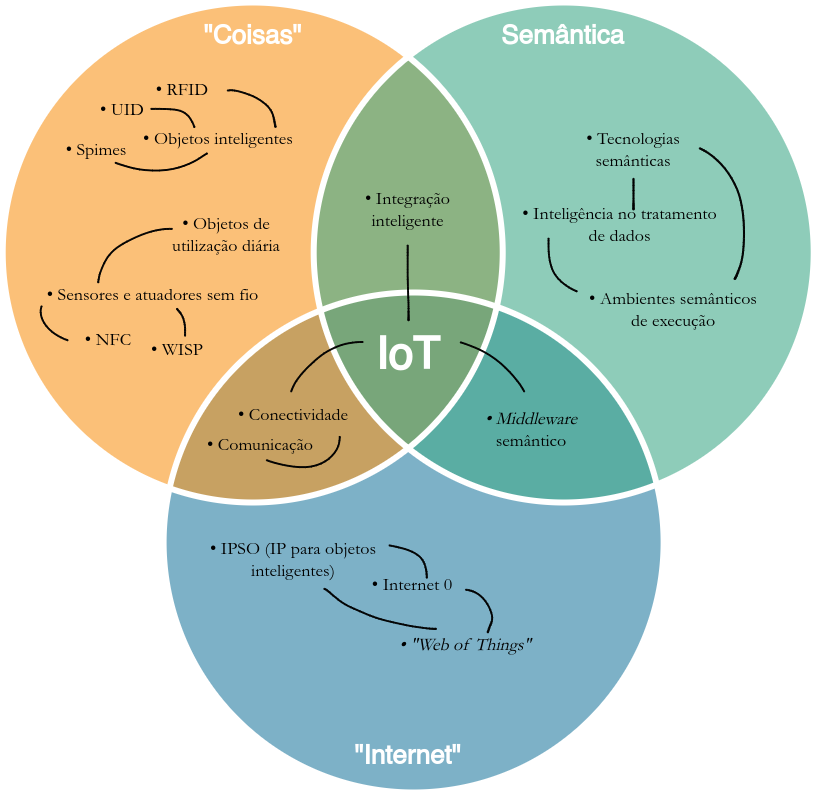
\includegraphics[width=0.7\linewidth]{USPSC-img/convergenceIoT2-low.png}
        \end{center}
        \fonte{adaptada de \cite{bandyopadhyay2011}}
    \end{figure}
    
    Para fortalecer o desenvolvimento no âmbito industrial, surgiu o \index{IIoT}IIoT como um novo tipo de ecossistema que envolve todos os domínios de logística, fabricação, gerenciamento e desenvolvimento. Concentra-se especificamente na aplicação da \index{IoT}IoT em ambientes industriais, viabilizando aprimoramentos em automação e eficiência e produtividade em variados setores (\textit{e.g.}, manufatura, energia, transporte e saúde). A Internet das Coisas Industrial não apenas envolve elementos de \textit{software} tradicionais, mas também requer controladores e sensores de \textit{hardware}, bem como plataformas de serviços em nuvem, para alcançar o domínio inteligente \cite{huichao2020}. A \autoref{fig:convergenceIIoT} ilustra a convergência dos tópicos de formação da \index{IIoT}IIoT.

    \begin{figure}[htbp]
        \caption{Convergência dos tópicos de formação da IIoT}
        \label{fig:convergenceIIoT}
        \begin{center}
            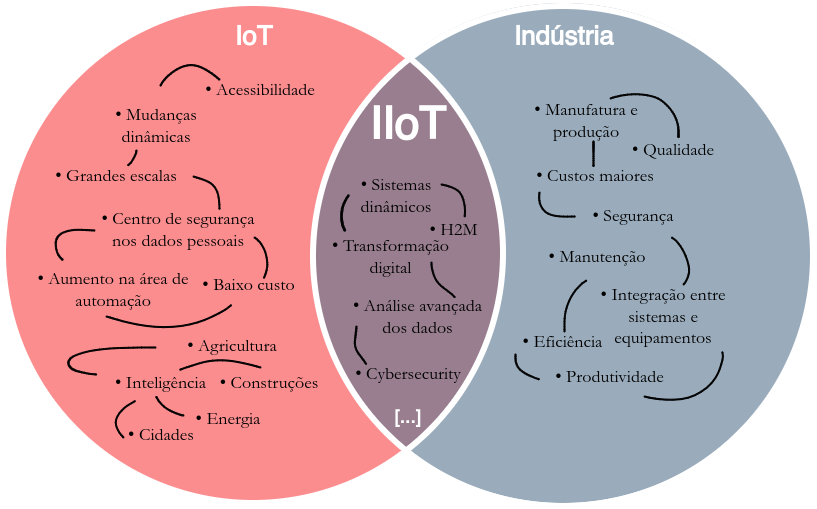
\includegraphics[width=0.7\linewidth]{USPSC-img/convergenceIIoT2-low.png}
        \end{center}
        \fonte{elaborada pelo autor.}
    \end{figure}
    
    Em sua escala, alcance e complexidade, a transformação digital, oriunda da atual revolução tecnológica, apresenta à sociedade desafios singulares ao alterar radicalmente nosso modo de viver e interagir. Intrinsecamente conectada à incessante troca de informações, ela atribui uma alta significância para as formas de transmissão, coleta e tratamento desses dados, que, cada vez mais abundantes, trazem informações mais completas e suficientes.

    Para que os dispositivos de transmissão de informações se comuniquem, uma linguagem formal deve ser especificada. De modo análogo à comunicação humana, estabelecer um diálogo compreensível torna-se uma tarefa árdua quando as partes envolvidas não compartilham o mesmo dialeto. Dessa forma, as linguagens especificam um conjunto de regras que asseguram uma comunicação cognoscível e a interoperabilidade entre sistemas, dispositivos e pessoas em diversos contextos.

    Tanto a \index{IoT}IoT quanto a \index{IIoT}IIoT dependem de protocolos robustos para estabelecer canais de comunicação confiáveis e seguros. Esses protocolos desempenham um papel crucial ao permitir o monitoramento, controle e gerenciamento em tempo real das implantações. Compreender os conceitos fundamentais e as características desses, é essencial para implementar e aproveitar efetivamente o potencial das tecnologias da (I)IoT.

    O termo protocolo, de acordo com \cite{persson2015}, caracteriza o conjunto de regras e orientações que redigem a comunicação e interação entre diferentes entidades ou sistemas, estabelecendo o formato, a ordem e o significado das mensagens trocadas. Projetado principalmente para garantir a interoperabilidade entre sistemas de vários fornecedores, um protocolo também simplifica a integração e o comissionamento de redes de comunicação de dados, reduzem os custos de instalação e permitem testes e validações independentes, o que, por sua vez, leva a projetos mais eficientes \cite{mohagheghi2009}.

    Os protocolos de comunicação existentes, tanto os originalmente projetados para ambientes industriais quanto os para a \index{IoT}IoT, não oferecem as características necessárias para a quantidade cada vez maior de dispositivos conectados \cite{markel2017}. Por essa razão, um novo conjunto de protocolos escaláveis e leves surgiu, dos quais se destacam o \index{OPC UA}OPC UA, MQTT, CoAP, entre outros. No entanto, neste trabalho, o protocolo \index{OPC UA}OPC UA é o único abordado, uma vez que representa o foco central desta investigação.
    
    \subsection{Principais Aspectos do Protocolo OPC UA} \label{subsec:opcUA}

        \textit{Open Platform Communications} (OPC, anteriormente conhecido como \textit{OLE for Process Control}), desenvolvido pela OPC Foundation, é um padrão de comunicação amplamente utilizado por vários anos nos mais diversificados setores da tecnologia da informação e automação industrial. De acordo com \citeonline{lange2010}, o OPC tem sido muito aceito nas últimas décadas como o padrão industrial mais popular entre usuários e desenvolvedores. A maioria dos fornecedores de IHM (Interface Homem-Máquina), SCADA (do inglês \textit{Supervisory Control and Data Acquisition}), e DCS (do inglês \textit{Distributed Control System}) da área, oferecem a tecnologia OPC como parte integrada de seus produtos.
        
        Duas etapas principais compõem o desenvolvimento desta tecnologia: (I) OPC Classic, e (II) \index{OPC UA}OPC UA. Em suma, o Classic fornece padrões de interface de comunicação neutros (no âmbito de fornecedores) para controle de processo e sistemas de automação de manufatura, incluindo acesso a dados (OPC DA), alarmes e eventos (OPC A\&E) e acesso a dados históricos (OPC HDA). Ele resolve a integração perfeita de dispositivos de campo, dispositivos de controle e sistemas de \textit{software} de automação (\textit{e.g.}, SCADA), melhorando a abertura e a interoperabilidade do sistema \cite{han2022}. No entanto, o produto desenvolvido na primeira etapa é limitado em sua capacidade de realizar aplicações integradas e em plataformas distintas e, principalmente, carece de tecnologias que o transformam em um protocolo de comunicação seguro. É por esse, e outros motivos, que a versão \textit{Unified Architecture} do OPC foi criada. Segundo \citeonline{lange2010}:
    
        \begin{citacao}
            O \index{OPC UA}OPC UA não foi planejado apenas como uma nova versão da interface padrão OPC, mas sim como uma nova visão de interoperabilidade "global" e troca de dados padronizada entre aplicações de \textit{software} independentes de fornecedores, linguagens de programação, sistemas operacionais e localização [...], ao implementar independência de plataforma, escalabilidade, alta disponibilidade, capacidade de Internet, entre outras características nesse novo protocolo.
        \end{citacao}
    
        Aproveitando as tecnologias de Serviços Web, XML e .NET, o UA é caracterizado por sua definição de objeto unificado e apresenta uma arquitetura completamente orientada a serviços (SOA, do inglês \textit{Service Oriented Architecture}). Também pode ser integrado com as mais recentes tecnologias, como: \textit{Time Sensitive Networking} (TSN) e 5G \cite{han2022}, e os dados de comunicação podem ser codificados usando diferentes métodos. Dentre as principais vantagens do protocolo, se destacam:
    
        \begin{itemize}
            \item \underline{Independência de plataforma}: por oferecer diferentes pilhas de \textit{software} em C/C++, .Net e Java, é possível desenvolvê-lo em vários sistemas e dispositivos embarcados, não limitando apenas à plataforma da Microsoft, como no OPC Classic;
            \item \underline{Mecanismos de segurança aprimorados}: inclui um conjunto completo de mecanismos de comunicação segura, na qual requer autenticação de duplo sentido para ambos os certificados e estabelecimento de canais seguros;
            \item \underline{Modo de acesso unificado aos dados}: ao integrar os dados atuais, notificações de eventos e histórico no mesmo espaço de endereço na modelagem de informações, o \index{OPC UA}OPC UA unifica as diferentes funções anteriores, por meio de apenas uma chamada;
            \item \underline{Suporte a estruturas de dados complexas}: as especificações existentes oferecem apenas uma organização hierárquica simples de itens, enquanto o \index{OPC UA}OPC UA oferece metamodelos de informações que podem ser facilmente estendidos, sendo possível incluir e excluir as ligações entre esses modelos de dados.
        \end{itemize}
        
        Todas as especificações lançadas pela OPC Foundation para o protocolo \index{OPC UA}OPC UA estão disponibilizadas em 24 partes, pela última versão de lançamento 1.05.02 do documento `OPC UA Specification' \cite{opc2022}. As partes 1 a 7 do documento apresentam as principais características da tecnologia, assim como o modo de segurança, espaço de endereçamento, conjunto de serviços, modelo de informação padrão, mapeamentos e perfis de serviço. As partes 8 a 13 estão relacionadas às definições de tipo de acesso a dados gerais padrão, como acesso a dados, alarmes e condições, programas, acesso histórico, descoberta e agregados. Alguns dos principais conceitos teóricos do protocolo concernentes para esta dissertação estão apresentados nas subseções abaixo, como o \textit{Address Space}, o \textit{Information Model}, a transmissão dos dados, a segurança implementada em cada camada e o processo de conexão entre um cliente e servidor OPC UA.
    
        \subsubsection{Espaço de Endereçamento e Modelo de Informação}

        Conceitua-se de forma concisa o Espaço de Endereço e Modelo de Informação (do inglês \textit{Address Space} e \textit{Information Model}) como, respectivamente, a fundação e componente central do \index{OPC UA}OPC UA. Pode-se equiparar esses dois conceitos, analogamente, à estrutura óssea e ao coração no corpo humano, na devida ordem supracitada. O \textit{Address Space} representa uma ampla variedade de informação, incluindo instâncias de objetos, variáveis e tipos \cite{gong2020}. O \index{OPC UA}OPC UA propõe um \textit{Address Space} consistente e um modelo de serviço, e isso ajudará a unificar dados, eventos e informações históricas no espaço de endereço do mesmo servidor \cite{ren2019}.
        
        Os \textit{Nodes} se caracterizam como os componentes em um Espaço de Endereço, sendo que cada um recebe uma classe correspondente a um elemento específico do modelo de objeto (do inglês \textit{Object Model}), incluindo variáveis, métodos e eventos. Essas classes servem coletivamente como os `metadados' do \textit{Address Space} e cada \textit{Node}, uma instância de uma classe. 
        
        A definição de classe contempla atributos e referências. Os Atributos (do inglês \textit{Attributes}) formam os componentes fundamentais de uma classe e cada definição de atributo inclui um ID, nome, descrição, tipo de dados e indicadores de obrigatoriedade. As referências (do inglês \textit{References}), por sua vez, indicam o relacionamento entre dois \textit{Nodes} conhecidos, e uma referência é determinada exclusivamente pelo nó de origem, o de destino, a semântica da referência e a sua direção.

        A \autoref{fig:opcuaArqCS} apresenta a arquitetura cliente-servidor do \index{OPC UA}OPC UA, ilustrando as conexões entre os conceitos supracitados.

        \begin{figure}[htbp]
            \caption{Arquitetura Cliente-Servidor do OPC UA}
            \label{fig:opcuaArqCS}
            \begin{center}
                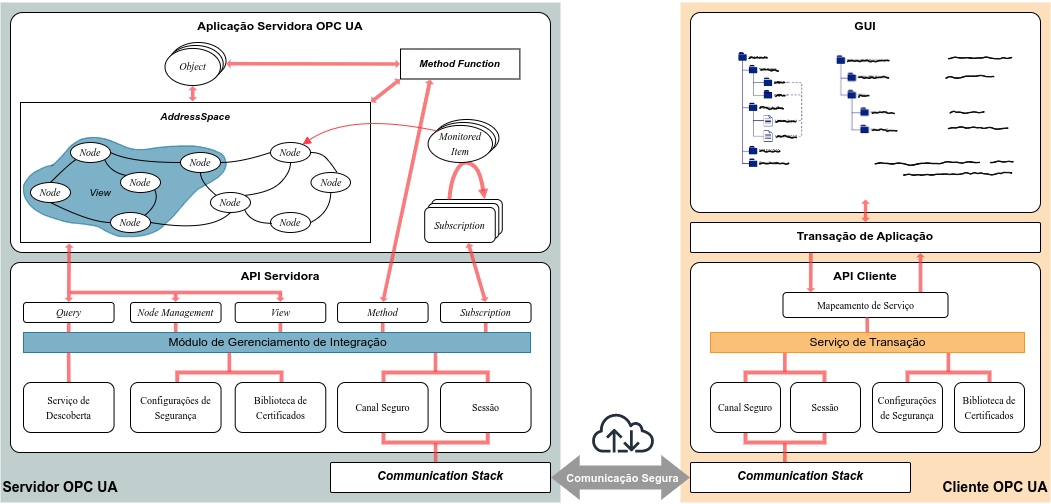
\includegraphics[width=1\linewidth]{USPSC-img/opcuaClientServerArc1-low.png}
            \end{center}
            \fonte{adaptada de \cite[Parte 6]{opc2022} e \cite{huang2010}.}
        \end{figure}

        O \textit{Information Model} é composto principalmente de \textit{Nodes} e \textit{References}, possibilitando a representação de diversas informações estruturadas e hierárquicas. Com funcionalidade abrangente orientada a objetos, até estruturas complexas de várias camadas podem ser modeladas e estendidas. O \index{OPC UA}OPC UA oferece uma estrutura de modelo fundamental e a possibilidade de criação de outros complementares para aplicações específicas, a fim de aprimorar ainda mais o sistema.

        A relação entre modelos de informação fundamental e específicos do usuário são representados na \autoref{fig:opcuaArq}. A aplicação \index{OPC UA}OPC UA apresenta a flexibilidade em seu desenvolvimento por poder ser iniciada a partir de um Modelo de Informação principal ou complementar padronizado que se alinha conforme o domínio específico. Com isso, aproveitando a abordagem de modelagem orientada a objetos do protocolo e utilizando o conjunto predefinido de serviços de acesso e manipulação, a interoperabilidade excepcional pode ser alcançada pelo sistema \cite{gong2020}.

        \begin{figure}[htbp]
            \caption{Infraestrutura de modelos do OPC UA}
            \label{fig:opcuaArq}
            \begin{center}
                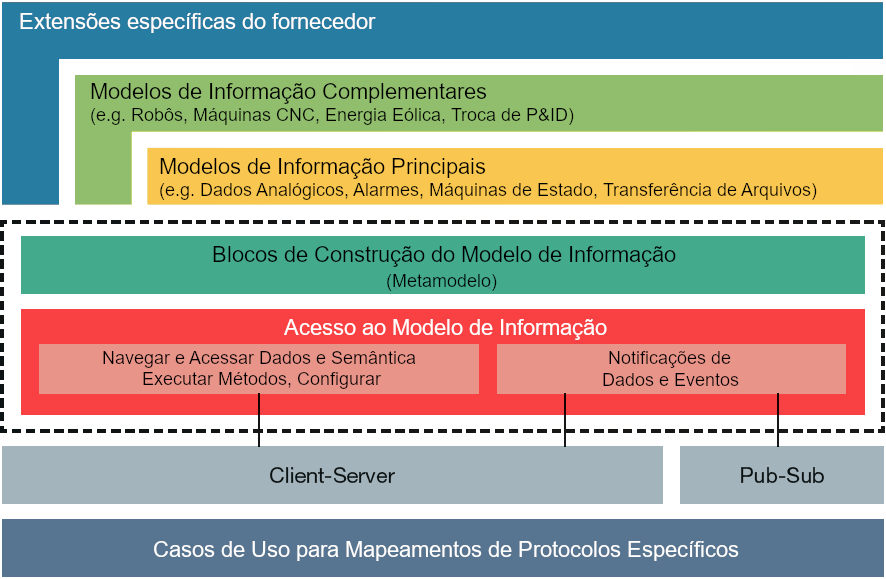
\includegraphics[width=0.9\linewidth]{USPSC-img/opcuaArq.png}
            \end{center}
            \fonte{adaptada de \cite{opc2019}.}
        \end{figure}

        \subsubsection{Métodos de Comunicação}

        O \index{OPC UA}OPC UA abrange mapeamentos de elementos independentes de protocolo para protocolos de transporte e segurança padronizados. Atualmente, a transmissão de dados pode ser realizada por meio de três métodos distintos: TCP/IP, SOAP/HTTP e HTTPS. Em termos de implementação de segurança, obrigatória para todas as variantes, o \index{OPC UA}OPC UA define \textit{UA Secure Conversation} e \textit{WS Secure Conversation} para TCP/IP e SOAP/HTTP, como os respectivos protocolos  \cite{neumann2015}.
        
        Em relação à codificação de mensagens e apresentações de dados, o \index{OPC UA}OPC UA oferece duas opções principais: UA-XML e UA-\textit{Binary}, nos quais utilizam, respectivamente, esquemas de codificação para Serviços Web e formatos binários, descritos na Parte 6 do documento de especificações \cite{opc2022}, para comunicação eficiente em sistemas de alta velocidade ou embarcados. Com isso, permitem flexibilidade na escolha do formato apropriado para transmissão e representação de dados eficientes. A \autoref{fig:ua-osi} ilustra essas abordagens do UA categorizadas no modelo de referência OSI (do inglês \textit{Open Systems Interconnection}), destacando os componentes de comunicação supracitados. %, sustentando a interoperabilidade e segurando do \index{OPC UA}OPC UA ao realizar um `desvio' por algumas camadas do modelo.
        
        \begin{figure}[htbp]
            \caption{Categorização da comunicação OPC UA no modelo de referência OSI}
            \label{fig:ua-osi}
            \begin{center}
                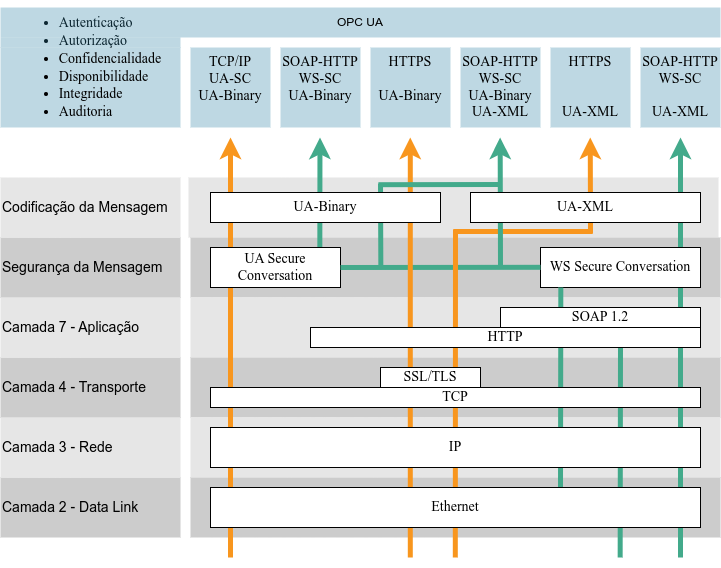
\includegraphics[width=0.9\linewidth]{USPSC-img/ua-osi-low.png}
            \end{center}
            \fonte{adaptada de \cite{neumann2015}.}
        \end{figure}

        \subsubsection{Escopo de Proteção}

        A segurança por muito tempo foi negligenciada, resultando no reconhecimento tardio de sua gravidade e na adoção vagarosa de medidas protetivas. Esse cenário foi especialmente evidenciado em ambientes industriais, cujas preocupações com segurança foram historicamente abordadas em conjunto com a \index{Tecnologia da Informação}TI. No entanto, à medida que a interconexão digital avança, a necessidade de proteção contra uma crescente gama de ataques cibernéticos em sistemas ciber-físicos tornou-se inegável, não apenas na camada de aplicação, mas em toda a infraestrutura desses ambientes críticos.
        
        O \index{OPC UA}OPC UA foi desenvolvido com foco na resolução desse problema histórico, ao tratar de questões desse tipo em diversas camadas. Seu escopo de proteção é dividido na segurança da informação pela tríade CIA (do inglês \textit{Confidentiality, Integrity and Availability}) e pelo \textit{Framework} AAA - autenticação, autorização e auditoria.
        
        Na camada de aplicação, a autenticação e a autorização do usuário são cruciais. Autenticar o acesso envolve a verificação da identidade do cliente usando métodos como: senhas, certificados X.509V3 ou \textit{tokens} de segurança, conforme supracitado. Por outro lado, autorizar esse acesso implica na sua concessão ou negação a serviços específicos. A documentação de especificação do protocolo não alude como os usuários devem autenticar ou autorizar seus direitos, no entanto, fornece os meios para tal implementação. As aplicações \index{OPC UA}OPC UA, tanto cliente quanto servidora, também devem se identificar durante o estabelecimento da comunicação segura usando certificados, permitindo aceite ou não da requisição.
        
        A camada de comunicação fornece um canal seguro através do qual os dados são transmitidos do cliente para o servidor. Essa mensagem secreta é utilizada para derivar as \textit{Symmetric Keys} do processo de criptografia dos dados requeridos e respondidos, garantindo a confidencialidade da comunicação ao impedir acessos não autorizados. Da mesma forma, a integridade é mantida por meio de assinaturas para verificar se as informações recebidas pelo cliente correspondem ao que foi enviado pelo servidor. A \autoref{subsubsec:conn} detalha o procedimento envolvido no estabelecimento do canal seguro entre servidor e cliente OPC UA.

        Por fim, as aplicações geram registros de auditoria que abrangem vários eventos, como tentativas de conexão, negociações de opções de segurança, alterações de configuração e sistema, interações do usuário e rejeições de sessão. O suporte a essas trilhas de auditoria de segurança é oferecido por meio de dois mecanismos: (I) a garantia da rastreabilidade entre os \textit{logs}, por meio de um identificador local na solicitação; e (II) a definição de parâmetros para inclusão nos registros de auditoria (parâmetros descritos pela Parte 5 das especificações).

        Mesmo com toda sua construção voltada para fortificar o sistema contra-ataques, o \index{OPC UA}OPC UA encontra desafios de segurança internos e externos, visto que a diversidade de protocolos na transmissão das mensagens herda os riscos de segurança dos mesmos. Assim, o estabelecimento de tecnologias robustas de segurança de rede é imperativo para lidar efetivamente com esses desafios.

        \subsubsection{Processo de Conexão Segura} \label{subsubsec:conn}

        O canal seguro estabelecido em uma comunicação OPC UA deve respeitar uma série de medidas no estabelecimento e no término da conexão, como a negociação de segurança, a decisão do algoritmo criptográfico e as políticas e perfis de segurança utilizados. A \autoref{fig:seqConn} apresenta o diagrama de sequências desse processo.

        \begin{figure}[htbp]
            \caption{Processo de criação e encerramento de conexão no OPC UA}
            \label{fig:seqConn}
            \begin{center}
                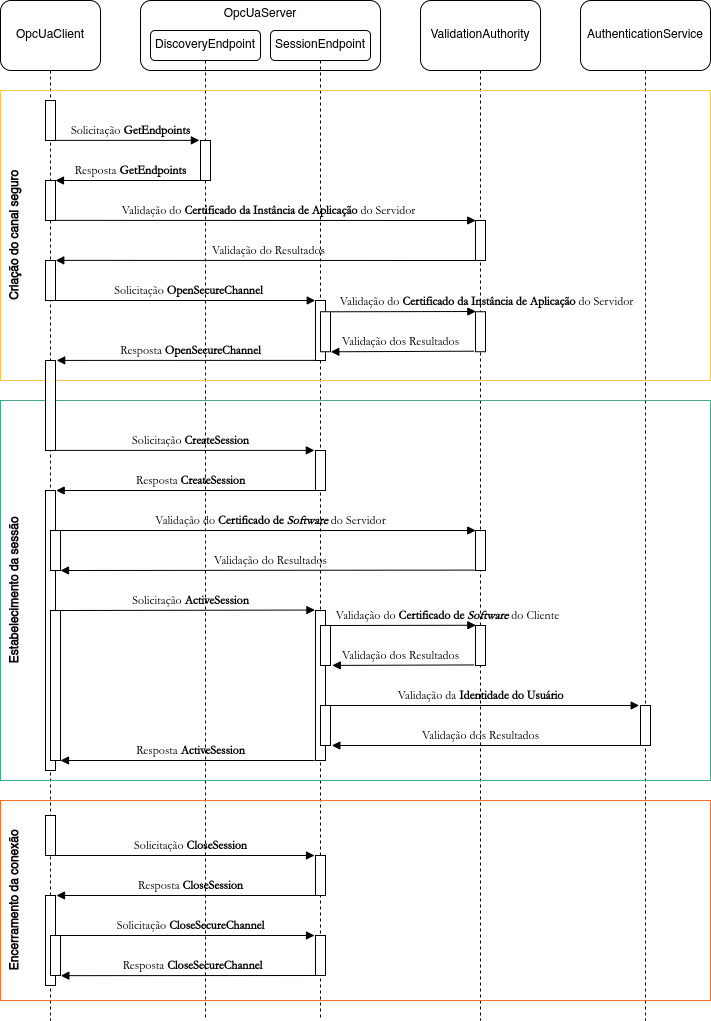
\includegraphics[width=0.972\linewidth]{USPSC-img/seqConn-low.png}
            \end{center}
            \fonte{adaptada de \cite{mahnke2009}.}
        \end{figure}

        Na etapa da criação da conexão, as diferentes opções de configuração do servidor são coletadas pelo cliente, caso esse não esteja pré-configurado. Uma solicitação \textbf{GetEndpoints} não segura é enviada do cliente ao \textbf{DiscoveryEndpoint} do servidor, a fim de obter as descrições dos \textbf{Endpoints} de sessão existentes, incluindo a configuração de segurança. Uma vez que essas informações são coletadas, o cliente seleciona o \textbf{Endpoint} e valida o certificado da instância de aplicação do servidor. 
        
        A segunda etapa ocorre caso o certificado seja considerado confiável após a validação. Uma solicitação \textbf{OpenSecureChannel} é criada e enviada ao \textbf{Endpoint} de sessão do servidor, incluindo a Política de Segurança e Modo de Segurança. O OPC UA incorpora um modelo de segurança flexível que consiste em três modos, descritos pelo \autoref{qdr:secureModes}.

        \begin{quadro}[htbp]
            \caption{\label{qdr:secureModes}Modos de segurança do OPC UA}
            \begin{tabular}{|M{3.60cm}|p{11.50cm}|}
                \hline
                \thead{Modos} & \thead{Descrição} \\
                \hline
                \textit{None}  & $\sbullet$ Nenhuma segurança \\
                \hline
                \multirow{4}{*}{\textit{Sign}} & $\sbullet$ Codificado com a chave privada do remetente \\
                    & $\sbullet$ Somente o proprietário do certificado possui a chave privada \\
                    & $\sbullet$ Qualquer pessoa pode verificar a identidade \\
                    & $\sbullet$ Fornece autenticidade \\
                \hline
                \multirow{5}{*}{\textit{Sign\&Encrypt}} & $\sbullet$ Adiciona criptografia para assinar \\
                    & $\sbullet$ Codificação com chave pública do receptor \\
                    & $\sbullet$ Qualquer pessoa pode criptografar \\
                    & $\sbullet$ Somente o proprietário do certificado pode ler \\
                    & $\sbullet$ Autenticidade, confidencialidade e integridade \\
                \hline
    	\end{tabular}
    	\begin{flushleft}
    		\fonte{adaptado de \cite{neu2019}.}
    	\end{flushleft}
        \end{quadro}

        Para lidar com a ameaça central da permissão de clientes maliciosos à rede, é possível alcançar a disponibilidade e a integridade do conteúdo das mensagens no modo seguro \textbf{Sign}, uma vez que as identidades dos servidores e clientes podem ser verificadas através da infraestrutura de chave pública e certificados. Para criptografar o conteúdo da comunicação de rede, utiliza-se o modo \textbf{Sign\&Encrypt}, garantindo também a confiabilidade desses dados.

        Assim sendo, uma sessão é instaurada com base no canal seguro criado pela conexão, mediante uma solicitação de \textbf{CreateSession} devidamente protegida pelo cliente. Na resposta dos servidores, por sua vez, são fornecidos os certificados de \textit{software}. A fase final do estabelecimento da comunicação é iniciada, então, após a validação bem-sucedida desses certificados por parte do cliente. Essa fase envolve a ativação da sessão criada através da solicitação \textbf{ActiveSession} ao servidor, cujas informações adicionais de credenciais do usuário e do \textit{software} estão contidas. A validação dos dados complementares representa o encerramento dessa composição de conexão, permitindo que o cliente acesse e comunique-se com o servidor exitosamente.

        O encerramento de uma conexão OPC UA ocorre por meio das solicitações \textbf{CloseSession} e \textbf{CloseSecureChannel}. A especificação do OPC UA \cite{opc2022} afirma que as mensagens de encerramento sejam apenas assinadas, pois nenhuma informação secreta é transmitida nessa etapa.

        % Os perfis (profiles) englobam a funcionalidade que uma aplicação suporta para estar em conformidade. Além disso, alguns perfis incluem funções de segurança, como o algoritmo de criptografia implementado. A escolha do mecanismo de segurança a ser usado é decidida mutualmente pelo cliente e pelo servidor. Ele é identificado por um URI e contém o nome exclusivo do algoritmo de segurança utilizado. Por exemplo, http:// opcfoundation.org/UA/SecurityPolicy#Basic128Rsa15, este URI define que o algoritmo AES com 128 bits é usado para criptografar e assinar mensagens de forma simétrica, e no caso de operação assimétrica, é usado o algoritmo RSA1.5. 2.2.1 Políticas de segurança OPC UA suportadas para Cliente-Servidor: • Aes128-Sha256-RsaOaep: Esta faceta de segurança define uma política de segurança que é usada quando há uma necessidade média de segurança. A infraestrutura de PKI é obrigatória para isso. À medida que o poder computacional aumenta, espera-se que as políticas de segurança expirem. O Instituto Nacional de Padrões e Tecnologia (NIST) ajuda a fornecer diretrizes sobre a data esperada de expiração da política de segurança. As diretrizes especificam a data em que a política deve ser atualizada ou se deve ser substituída por um algoritmo mais seguro. Embora as diretrizes não mencionem se o algoritmo falhou. Esta política de segurança em particular não tem data de término até o momento [15]. • Aes256-Sha256-RsaPss: Esta política de segurança é usada quando há uma alta necessidade de segurança. A infraestrutura de PKI é obrigatória para isso. O NIST fornece as mesmas diretrizes para esta política de segurança, mencionando a data de expiração junto com a necessidade de atualização ou substituição da política por uma mais segura [15]. • Basic128Rsa15 (obsoleta): Esta política de segurança é usada quando se necessita de segurança média. A infraestrutura de PKI é necessária também. O NIST fornece as mesmas diretrizes para esta política de segurança. O NIST recomendou aos usuários desta política que atualizassem as chaves com menos de 2048 bits em 2010. Além disso, eles também recomendaram em 2012 que as políticas usando chaves com menos de 2048 bits fossem descontinuadas. A partir da Especificação OPC UA Versão 1.04, esta política de segurança foi descontinuada, uma vez que o algoritmo de hash SHA1 não é mais considerado seguro. Se o servidor incluir esta política de segurança, ela deve ser desabilitada por padrão e será fornecida documentação descrevendo que ela não deve mais ser utilizada [15]. • Basic256 (obsoleta): Assim como a Basic128Rsa15, esta política de segurança também foi descontinuada na Especificação OPC UA Versão 1.04. A razão pela qual isso foi descontinuado foi a mesma, uma vez que o algoritmo de hash SHA1 não era mais considerado seguro [15]. • Basic256Sha256: Esta política de segurança é usada quando o sistema requer altos níveis de segurança. Isso requer infraestrutura de PKI. O NIST fornece as mesmas diretrizes que anteriormente. Também é recomendado que os Servidores e o Cliente suportem todos os perfis de segurança e que os desenvolvedores forneçam o perfil recomendado como padrão [15]. • None: Esta Faceta de segurança define uma política de segurança usada para configurações com as menores necessidades de segurança. Isso pode afetar o comportamento dos Serviços CreateSession e ActivateSession. Se esta política de segurança for usada, o SecureChannel criado não terá segurança de canal. De acordo com a documentação, se houver outra política de segurança disponível, ela deve ser desativada por padrão [15].
        
    \section{\textit{Cybersecurity}} \label{sec:cybersecurity}

    No passado, os setores de \index{Tecnologia da Informação}tecnologia da informação e \index{Tecnologia Operacional}tecnologia operacional eram organizacionalmente separados. Atualmente, a transformação digital está pressionando a indústria a reconsiderar esse paradigma e implantar projetos de convergência que unam \index{Tecnologia da Informação}TI e \index{Tecnologia Operacional}TO em um mesmo conceito. A \autoref{fig:convIT/OT} apresenta os principais tópicos abordados na \index{Convergência TI/TO}convergência TI/TO. Essa convergência não está apenas gerando um desafio complexo em termos de comunicação de dados, mas também enfrentando uma classificação de preocupações de \index{Segurança Cibernética}segurança cibernética \cite{wiboonrat2022}.

    \begin{figure}[htbp]
        \caption{\label{fig:convIT/OT}Tópicos da convergência TI/TO}
        \begin{center}
            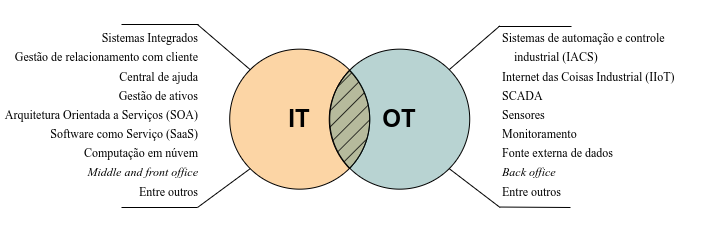
\includegraphics[width=1\textwidth]{USPSC-img/convergenceITOT-low.png}
        \end{center}
        \legend{Fonte: adaptado de \cite{yassine2021}.}
    \end{figure}

    Os Sistemas de Automação e Controle Industrial abrangem vários tipos de sistemas, incluindo SCADA, DCS (do inglês \textit{Distributed Control System}), CLP (Controlador Lógico Programável), sistemas de monitoramento, entre outros. A \index{Convergência TI/TO}convergência TI/TO tornou os \index{IACS}IACS mais complexos, poderosos e produtivos. Por outro lado, introduziu também novas \index{Vulnerabilidade}vulnerabilidades a potenciais acidentes e incidentes relacionados com a segurança, aumentando drasticamente seu risco associado. Esses sistemas são alvos cada vez mais frequente de ataques devido ao valor dos dados e à sua importância crítica para a economia. O \autoref{qdr:it-iacs} resume os resultados da comparação das principais características e objetivos de segurança do IACS com os do sistema de TI.
    
    \begin{quadro}[htbp]
        \caption{\label{qdr:it-iacs}Diferenças dos sistemas de TI e o IACS}
        \begin{tabular}{|M{3.25cm}|p{5.50cm}|p{5.50cm}|}
            \hline
             & \thead{TI} & \thead{IACS} \\
            \hline
            \multirow{12}{*}{\shortstack{Ambiente de \\ configuração}} & $\sbullet$ Equipamento padronizado & $\sbullet$ Equipamentos especializados conforme o processo \\
            & $\sbullet$ Ciclo curto de reposição de equipamentos & $\sbullet$ Poucos ciclos de substituição de equipamentos \\
            & $\sbullet$ Fácil de corrigir e reparar & $\sbullet$ Difícil de corrigir e reparar devido à disponibilidade do equipamento \\
            & $\sbullet$ Use um sistema operacional universal & $\sbullet$ SO de uso geral personalizado ou operação de SO autodesenvolvido\\
            & $\sbullet$ Velocidade e desempenho da rede & $\sbullet$ A comunicação de rede em tempo real é importante\\
            \hline
            \multirow{5}{*}{\shortstack{Objetivos Críticos \\ de segurança}} & $\sbullet$ Bloqueio o vazamento de dados importantes e a interrupção do serviço & $\sbullet$ Bloqueio da possibilidade de interrupção da produção e do processo \\
            & & $\sbullet$ Prevenção de acidentes pessoais em caso de acidentes \\
            \hline
            \multirow{4}{*}{\shortstack{Efeito nas ameaças \\ à segurança}} & $\sbullet$ Danos causados pelo vazamento de dados importantes & $\sbullet$ Danos diretos causados pela produção e vítimas humanas \\
            & $\sbullet$ Questões legais e danos à confiança da empresa & $\sbullet$ Danos à confiabilidade do produto \\
            \hline
	\end{tabular}
	\begin{flushleft}
		\fonte{adaptado de \cite{shin2022}.}
	\end{flushleft}
    \end{quadro}

    Em 2022, a equipe de resposta a emergências cibernéticas em sistemas de controle industriais da Kaspersky (Kaspersky ICS CERT) revelou o estado atual e os desafios da \index{Segurança Cibernética}segurança cibernética industrial em seu relatório de \index{Ameaça Cibernética}ameaças para sistemas de automação industrial \cite{kaspersky2023} ao registrar 1.198.532 ataques, representando um aumento de 16,2\% em relação ao ano anterior. Os ataques de \textit{ransomware} e as \index{Ameaça Cibernética}ameaças persistentes avançadas (APT, do inglês \textit{Advanced Persistent Threat}) foram as principais preocupações para os \index{IACS}IACS durante o período analisado.

    Adicionalmente, um estudo conduzido por \citeonline{corallo2022} destacou a \index{Segurança Cibernética}segurança cibernética como mais premente na adoção da \index{IIoT}IIoT. Isso sublinha a necessidade imperativa de que as empresas da área, juntamente com outros fatores críticos, como \textit{Big Data}, \index{Inteligência Artificial}Inteligência Artificial e \index{Software}\textit{Software} de Código Aberto, coloquem a segurança cibernética no centro de suas prioridades, evidenciando a complexidade e a relevância crescente da segurança digital no cenário industrial atual.

    De acordo com \citeonline{baybulatov2022}, a avaliação do risco de \index{Segurança Cibernética}segurança cibernética de um sistema pode ser derivada como a interseção de três elementos: ativos, \index{Vulnerabilidade}vulnerabilidades e \index{Ameaça Cibernética}ameaças. Na perspectiva de um \index{IACS}IACS, ativos são objetos cibernéticos relacionados ao controle industrial -- componentes de \textit{hardware} e \textit{software} -- e devem ser protegidos pelo sistema. \index{Vulnerabilidade}Vulnerabilidades são pontos fracos de ativos que podem ser explorados por \index{Ameaça Cibernética}ameaças. Por sua vez, \index{Ameaça Cibernética}ameaças são potenciais ações intencionais negativas ou eventos acidentais facilitados por \index{Vulnerabilidade}vulnerabilidades, que resultam em impactos indesejáveis. Os \index{IACS}IACSs apresentam \index{Vulnerabilidade}vulnerabilidades específicas que precisam ser abordadas para garantir a \index{Segurança Cibernética}segurança cibernética, das quais se destacam: 

    \begin{itemize}
        \item \underline{Rede}: a composição obrigatória de redes de comunicação nos sistemas \index{IACS}IACSs os tornam suscetíveis às várias \index{Ameaça Cibernética}ameaças, uma vez que, devido à interconectividade, as \index{Vulnerabilidade}vulnerabilidades também são herdadas. Devido à dificuldade de atacarem diretamente o destino, os invasores encontram, na maioria das vezes, \index{Vulnerabilidade}vulnerabilidades na rede \index{IACS}IACS como ponto de partida, alcançando assim o host de destino por meio dessa conectividade \cite{li2020}.
        \item \underline{\textit{Software} e \textit{Firmware}}: a maioria dos sistemas de automação e controle industriais personalizam esses componentes em suas instalações. O desenvolvimento e gerenciamento incorreto desses, como falhas de codificação, inserção de código malicioso ou falta de atualizações de segurança, introduzem \index{Vulnerabilidade}vulnerabilidades de segurança no sistema. Além disso, organizações desse meio enfrentam desafios na aplicação de atualizações de \textit{softwares} e \textit{firmwares} devido à necessidade de minimizar as interrupções operacionais. No entanto, os sistemas que executam um \textit{software} afetado estão mais sujeitos a ataques e explorações, que são geralmente expostas mais rapidamente \cite{maidl2021}.
        \item \underline{Falta de profissionais qualificados}: os engenheiros e especialistas que projetam um \index{IACS}IACSs dominam normalmente o \textit{hardware} e \textit{software} de controle no aspecto de aplicação. Há uma lacuna no treinamento com relação à implementação de segurança eficaz usando os recursos existentes dos componentes de uma \index{IACS}IACS, sem mencionar os últimos aprimoramentos de \index{Segurança Cibernética}segurança cibernética \cite{graham2016}. Devido a esta falta de qualificação, as configurações desenvolvidas podem incluir senhas fracas, permissões excessivas, configurações de rede inseguras ou falta de segregação de redes.
    \end{itemize}

    Apesar disso, existem diversas normas que oferecem suporte para focar e mitigar \index{Vulnerabilidade}vulnerabilidades de segurança atuais e futuras, como as séries ISA/IEC 62443 - definida como a estrutura internacional de padrões de \index{Segurança Cibernética}segurança cibernética para \index{Tecnologia Operacional}TO. A estrutura compreende uma coleção de padrões, relatórios técnicos e informações relacionadas para a proteção de um \index{IACS}IACS, além de defender todas as partes relacionadas à \index{Segurança Cibernética}segurança cibernética desses sistemas com orientação e uma base comum para medidas técnicas e organizacionais, a fim de aumentar a resiliência digital \cite{wiboonrat2022}. 

    Adicionalmente, diversas medidas de proteção desempenham um papel fundamental no aprimoramento da segurança de um IACS, como a segmentação da rede, autenticação e controle de acesso, \index{SDI}SDI, SIEM, UTM, entre outras. Entretanto, os Sistemas de Detecção de \index{Intrusão}Intrusão (\index{SDI}SDI) se destacam como uma das mais eficazes. Essa tecnologia consegue monitorar comunicações anormais e melhorar o gerenciamento de segurança de uma determinada rede \cite{shi2021}. % A \autoref{subsec:sdi} apresenta os principais conceitos relacionados aos \index{SDI}SDI, como arquiteturas e métodos de detecção.

    Diante desse cenário, proteger esses sistemas contra \index{Ameaça Cibernética}ameaças cibernéticas torna-se uma prioridade essencial para garantir a continuidade das operações, a disponibilidade dos dados, a segurança dos envolvidos, a proteção do meio ambiente e a confiabilidade dos produtos e serviços oferecidos pelas indústrias. A implementação de medidas robustas de \index{Segurança Cibernética}segurança cibernética, juntamente com a adoção de práticas recomendadas e a conformidade com as normas e regulamentações pertinentes são fundamentais para mitigar os riscos e fortalecer a resiliência dos sistemas industriais. % A \autoref{subsec:tiposAtaques} aborda os principais tipos de ataques em redes industriais e suas classificações.

    \subsection{Ataques em Redes Industriais} \label{subsec:tiposAtaques}

    A utilização das redes de comunicação em \index{IACS}IACS acrescenta novas \index{Vulnerabilidade}vulnerabilidades a \index{Ataque Cibernético}ataques ciber-físicos, podendo até prejudicar os processos físicos desses sistemas. Segundo \cite{turcato2020}, os ataques são também considerados \index{Anomalia}anomalias na rede e podem ser identificados principalmente por meio do fluxo do tráfego de dados. Esses ataques compreendem um “conjunto de ações ilícitas que tentam comprometer a integridade, confidencialidade, ou disponibilidade de recursos na rede”.

    No entanto, para um correto compreendimento acerca dos ataques em redes industriais, é necessário apresentar inicialmente o contexto desse termo. Os \index{Ataque Cibernético}ataques cibernéticos causam \index{Anomalia}anomalias no comportamento dos processos observados (na dinâmica das séries temporais de dados) durante a operação do \index{IACS}IACS. Essas \index{Anomalia}anomalias podem ser definidas pelo comportamento diferente da operação normal do tráfego da rede.

    As \index{Anomalia}anomalias podem ser maliciosas ou não intencionais, mas o conhecimento e análise delas deve ocorrer em todos os casos, pois possibilitam o congestionamento da rede e até um impacto ao processo industrial. Vale ressaltar que nem toda \index{Anomalia}anomalia pode ser considerada um \index{Ataque Cibernético}ataque cibernético, mas o contrário é correto. De acordo com \cite{barford2002}, as \index{Anomalia}anomalias podem ser classificadas em quatro categorias:

    \begin{itemize}
        \item \underline{\index{Anomalia}Anomalias na operação}: ocorrem a partir de uma falha ou problema de funcionamento da rede, por exemplo, a interrupção na operação normal, congestionamentos, indisponibilidade de dispositivos, configuração inadequada de um componente ou adição não programada de um mesmo; 
        \item \underline{\index{Anomalia}Anomalias \textit{flash-crowd}}: representam um aumento repentino no tráfego da rede devido a eventos ou circunstâncias excepcionais, como uma abundância de pacotes oriundos de uma estação para um CLP;
        \item \underline{\index{Anomalia}Anomalias na medição}: surgem com a presença de erros ou falhas nos métodos de medição utilizados para monitorar o desempenho da rede, gerando assim, uma análise imprecisa ou distorcida das informações;
        \item \underline{Ataques}: anomalia resultante de atividades maliciosa direcionada à rede.
    \end{itemize}

    % A detecção de tentativas não autorizadas de acesso à rede \index{IACS}IACS e destes outros tipos de \index{Anomalia}anomalias supracitados, também são componentes críticos da \index{Segurança Cibernética}segurança cibernética atualmente, mas estão fora do escopo deste trabalho.

    Por compreenderem um conjunto de ações ilícitas efetuadas visando comprometer algum dos pilares de uma comunicação segura (CIA), os ataques em redes de comunicação podem adulterar as informações, não respeitar alguma regra de privacidade e tornar indisponível e não confiável a infraestrutura da rede. O sucesso desses ocorre devido às \index{Vulnerabilidade}vulnerabilidades ou possíveis falhas nos elementos da rede, como configurações inadequadas ou erros no desenvolvimento.

    Inúmeros \index{Ataque Cibernético}ataques cibernéticos foram testemunhados nos últimos anos contra \index{IACS}IACS. Alguns desses ataques estão listados no \autoref{qdr:cyberattacks}. Tais incidentes históricos destacam as terríveis consequências que uma violação de segurança ou comprometimento do \index{IACS}IACS pode ter na economia e na segurança pública, assim como a correlação desses com a falta de segurança dos protocolos de comunicação. Embora esse cenário esteja mudando, com vários protocolos industriais sendo redesenhados, esse assunto continua sendo um problema, pois os protocolos legados ainda são amplamente utilizados. Além disso, uma das lições aprendidas com os ataques históricos é que, com tempo suficiente, invasores determinados e com bons recursos provavelmente podem obter acesso a quase todo sistema.
    
    \begin{quadro}[htbp]
        \caption{\label{qdr:cyberattacks}Principais ataques cibernéticos industriais dos últimos anos}
        \begin{tabular}{|p{1.00cm}|p{4.25cm}|p{2.00cm}|p{7.00cm}|}
            \hline
            \thead{Ano} & \thead{Alvo} & \thead{Local} & \thead{Descrição} \\
            \hline
            2000 & Instalação de tratamento de água `Maroochy Shire' & Austrália & Um dos primeiros relatórios de danos às instalações \index{IACS}IACS devido a \index{Ataque Cibernético}ataques cibernéticos, no qual causou a liberação de mais de 265.000 galões de esgoto não tratado \cite{sayfayn2017}. \\
		\hline
            2010 & Instalações nucleares & Irã & Conhecido como "a primeira arma digital publicamente conhecida do mundo", o STUXNET  foi um \textit{worm} de computador altamente sofisticado e malicioso desenvolvido para atacar um \index{IACS}IACS \cite{schneier2013}. \\
		\hline
            2012 & Instalações de energia & Oriente médio & O \textit{malware} Shamoon costumava atingir grandes empresas de energia no Oriente Médio, incluindo a Saudi Aramco e a RasGas \cite{nytimes2012}. \\
            \hline
            2016 & Sistema elétrico & Ucrânia & Com esse ataque, 30 subestações de energia foram derrubadas por seis horas, afetando cerca de 80000 pessoas \cite{cbc2016}. \\
            \hline
		2021 & Sistema de oleoduto & Estados Unidos & Colonial Pipeline, empresa que comporta um dos maiores oleodutos dos Estados Unidos, foi forçada a fechar seu oleoduto após ser atingida por um ataque de \textit{ransomware} \cite{nytimes2021}. \\
		\hline
            2021 & Sistema de abastecimento de água & Estados Unidos & Um hacker tentou envenenar o abastecimento de água em uma comunidade da Flórida que atende 15.000 pessoas \cite{hall2021}. \\
            \hline
	\end{tabular}
	\begin{flushleft}
		\fonte{elaborado pelo autor.}
	\end{flushleft}
    \end{quadro}

    \citeonline{sayegh2013} complementam documentando uma ampla gama de ataques ao \index{IACS}IACSs, a fim de descobrir como o sistema e diversos protocolos respondem a diversos tipos de ataques (\textit{e.g.}, negação de serviço (DoS)), assim como avaliar o grau de proteção e \index{Vulnerabilidade}vulnerabilidades desses.

    Uma taxonomia de \index{Ataque Cibernético}ataques ciber-físicos é proposta por \citeonline{teixeira2012}, baseando-se em três dimensões: (I) conhecimento do adversário sobre o sistema -- representa ataques poderosos que permitem a evasão dos adversários --, (II) grau de perturbação -- a capacidade de um adversário em afetar o sistema de destino violando sua integridade ou disponibilidade -- e (III) grau de divulgação -- a capacidade do adversário de obter informações confidenciais durante o ataque, por exemplo, violando dados ou controlando a confidencialidade.

    Segundo estatísticas do Centro de Estudos, Resposta e Tratamento de Incidentes de Segurança no Brasil \cite{cert2023}, o número de ataques aumenta significativamente com o passar dos anos. A \autoref{fig:certbr} apresenta, graficamente, os incidentes notificados ao CERT.br nos últimos 10 anos.

    \begin{figure}[htbp]
        \caption{\label{fig:certbr} Notificações de Incidentes recebidos pelo CERT.br nos últimos 10 anos}
        \begin{center}
            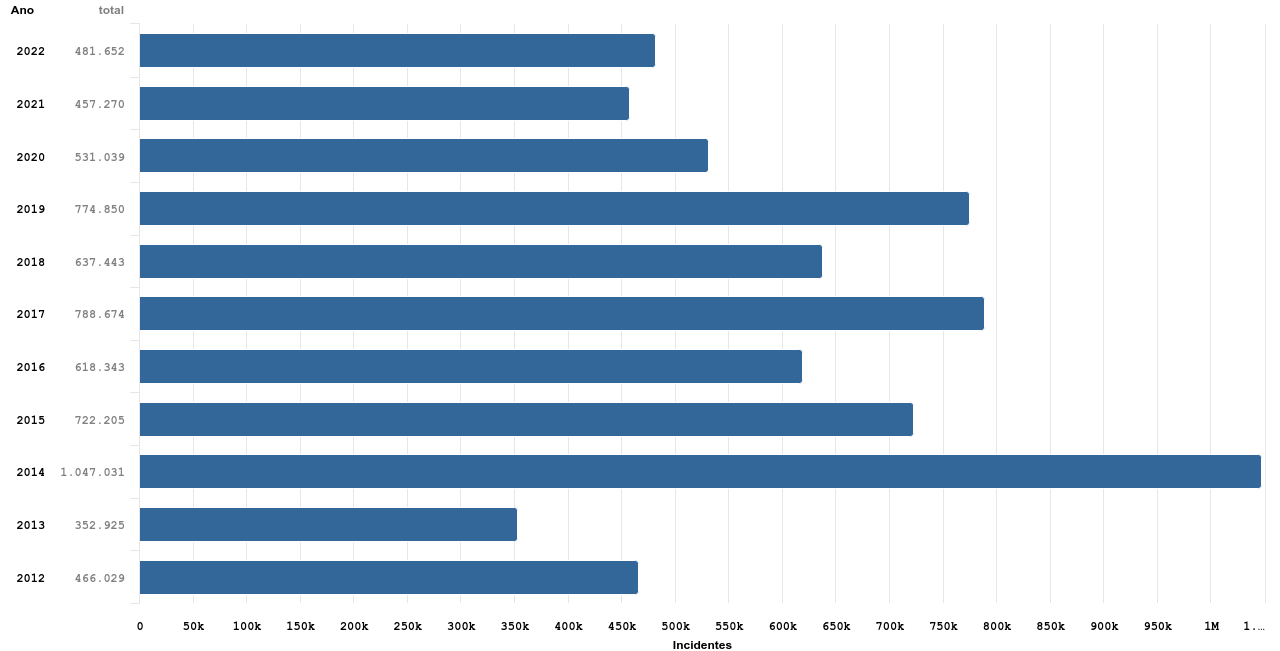
\includegraphics[width=1\textwidth]{USPSC-img/certbr.png}
        \end{center}
        \legend{Fonte: \cite{cert2023}}
    \end{figure}

    Os ataques podem ser classificados de diversas formas. A classificação base pode ser observada no glossário proposto por \citeonline{shirey2007}, cujos critérios são a origem, o destino ou alvo e objetivos do ataque. Todavia, algumas taxonomias foram propostas a fim de aprimorar essa classificação, como o modelo AVOIDIT \cite{simmons2009} -- classificando um ataque pelo seu vetor, impacto operacional, defesa, impacto informativo e alvo -- e o modelo TAVI \cite{drias2015} -- no qual divide a classificação pela \index{Ameaça Cibernética}ameaça, objetivo, \index{Vulnerabilidade}vulnerabilidade e impacto do ataque.

    Quanto à origem, os ataques podem ser externos ou internos. Os externos são aqueles disparados por um atacante de fora da rede, enquanto os internos são aqueles provenientes de usuários internos à rede que abusam de seus direitos e privilégios para realizar atividades não autorizadas \cite{turcato2020}.

    Já para a classificação com base no alvo, o ataque é realizado à rede, afetando a camada de comunicação ao impedir a utilização de alguns recursos da rede, ou ao sistema na totalidade, alterando senhas e configurações críticas dos equipamentos.
    
    No ponto de vista da classificação pelo objetivo, existem dois tipos principais de ataques que um invasor pode realizar:

    \begin{itemize}
        \item \underline{Passivo}: o intruso apenas `escuta' a comunicação, silenciosamente, sem qualquer alteração na comunicação. Tal espionagem ou análise de tráfego pode ocasionar a quebra da confidencialidade da informação, consistindo assim em crime contra a privacidade;
        \item \underline{Ativo}: refere-se à modificação de mensagens e fluxo de dados reais ou geração de dados falsos na comunicação. Afeta a integridade e confidencialidade dos dados, uma vez que o intruso pode repetir fluxos de dados antigos, alterando as mensagens de comunicação ou removendo alguma parte selecionada de mensagens importantes de comunicação. Os ataques ativos mais frequentes a redes posem ser classificados como: R2L (\textit{Remote to Local}) e U2R (\textit{User to Root}).
    \end{itemize}

    O \textit{Sniffing} de pacotes representa um ataque passivo em relação ao objetivo, uma vez que não envolve a modificação ou interrupção direta do tráfego de rede. Consiste em uma técnica aplicada para a captura e inspeção minuciosa dos pacotes em uma conexão estabelecida, sem que os agentes da comunicação estejam cientes da interceptação. Vale ressaltar que, enquanto o \textit{Sniffing} em si não causa alterações no tráfego ou nos dados, as informações obtidas podem ser posteriormente exploradas em ataques subsequentes. Por outro lado, o ataque \textit{Probing} é realizado de forma ativa, apesar de não comprometer o sistema. Envolve uma varredura do mesmo por parte do invasor pelo envio de requisições ao alvo, visando identificar entradas do sistema ou \index{Vulnerabilidade}vulnerabilidades para posteriormente explorar as fraquezas encontradas.
    
    No ataque DoS, uma sobrecarga do sistema ou rede é ocasionada por meio de solicitações excessivas do invasor, resultando em um esgotamento dos recursos computacionais ou de memória dos equipamentos. Com isso, os componentes da rede ficam impossibilitados de executarem suas tarefas devido ao envio de uma quantidade de informações superior ao que o sistema possa manipular (\textit{flooding}), assim como algumas \index{Vulnerabilidade}vulnerabilidades podem ser expostas a partir desse tipo de ataque ativo (exploração de falhas). Há a possibilidade desse ataque ser realizado em série, cujos invasores utilizam de vários locais para lançar o ataque, classificando-o assim como DDoS (do inglês \textit{Distributed DoS}). Um exemplo de DoS no âmbito industrial é um cujo invasor envia um comando para desligar a CPU de um CLP, exigindo a execução de um \textit{hard-reset} do dispositivo para retorno. Uma vez desligada, o CLP não pode se comunicar ou processar qualquer informação, resultando em uma `negação de serviço'.

    Quando ocorre a obtenção não autorizada de dados confidenciais de comunicação, caracteriza-se um ataque do tipo \textit{Man-In-The-Middle} (MITM), também conhecido como "Espionagem" (do inglês \textit{Eavesdropping}). Essa ação maliciosa pode resultar em uma significativa violação de segurança ou no comprometimento das informações, o que, por sua vez, pode abrir caminho para ataques subsequentes. Em um cenário Cliente-Servidor, caso o invasor já tenha comprometido o canal de comunicação, ele tem a capacidade de gravar e capturar as mensagens, afetando assim a confidencialidade dos dados. Além disso, uma vez estabelecida a sessão, tanto a autorização quanto a autenticação podem ser impactadas.

    Nos ataques de penetração, conhecidos como R2L e U2R, aquisições ou alteração não autorizada dos privilégios, recursos ou dados do sistema, violando as propriedades de integridade e controle dos recursos e dados. Com esses ataques, pode-se ganhar controle de um sistema ao explorar uma variedade de falhas de \textit{software} \cite{turcato2020}. A categoria R2L se destaca pelo envio de pacotes por uma rede externa, a fim de explorar privilégios de um usuário local. Já na U2R, os invasores conseguem acesso na rede local, e nesse cenário, tenta explorar as \index{Vulnerabilidade}vulnerabilidades para obter privilégios adicionais.

    % As características, a complexidade e a crescente sofisticação dos ataques faz com que aumente a demanda por técnicas de detecção mais precisas para o monitoramento contínuo da rede de comunicação industrial. Tais técnicas devem ser capazes de lidar com novos tipos de ataques e integrar-se facilmente aos demais mecanismos de proteção da rede sem sobrecarregar a comunicação \cite{maglaras2014}.

    De acordo com \cite{cekerevac2017}, o ataque MITM e DoS são os tipos mais comuns de ataque que a IIoT enfrenta, sendo responsáveis por quase 64\% dos ataques. Com o aumento da interconectividade entre sistemas nas indústrias, o ataque MITM está se tornando um desafio maior, pois é mais fácil para o invasor obter acesso a informações confidenciais através dele. Quando se trata de DoS, além de ser também comumente empregado, pode agir de maneira ativa no sistema, gerando perdas consideráveis para as indústrias. Neste projeto, três ataques são aplicados em uma rede industrial OPC UA: \textit{sniffing} de pacotes, MITM e DoS.
    
    % \subsection{Modelagem de Ameaças} \label{subsec:modAmeaca}

    \subsection{Análise e Descoberta de Vulnerabilidades} \label{subsec:analVul}

    Inúmeros empreendimentos de pesquisa têm sido dedicados à análise das origens de erros presentes em sistemas computacionais e \textit{softwares} (popularmente denominados \textit{bugs}). Visando a minimização das ocorrências desses erros nos sistemas e o desenvolvimento de métodos para avaliar a existência, esses estudos apresentam, ordinariamente, ferramentas para a identificação de \textit{bugs} específicos.

    Apesar da implementação de várias técnicas e tecnologias, esses erros intrínsecos ao desenvolvimento persistem. As vulnerabilidades surgem quando os \textit{bugs} comprometem a integridade do sistema ou políticas de segurança, podendo ser mensurada pelo grau em que um sistema, subsistema ou componente do sistema tem probabilidade de sofrer danos devido à exposição a um perigo.

    As vulnerabilidades podem ser amplamente difundidas e consistentes em vários sistemas. Erros de desenvolvimento, equívocos de configuração e falhas operacionais, frequentemente, servem como porta de entrada para usuários não autorizados, permitindo que efetuem ações maliciosas: expor/alterar informações confidenciais, interromper/destruir um sistema ou assumir o controle de um sistema/\textit{software} \cite{dowd2006}. Um estudo realizado por \citeonline{shin2022} revela que 92\% dos sistemas que utilizam o protocolo OPC UA estão inadequadamente configurados devido a diversas falhas, como a ausência de controle de acesso, a desativação de funcionalidades de segurança, a utilização de políticas criptográficas obsoletas e a reutilização de certificados. Essa alta porcentagem de inadequações é atribuída principalmente à complexidade das configurações de segurança intrínsecas ao protocolo.
    
    A análise de vulnerabilidades engloba a formulação de uma categorização, ou conjunto destas, que viabiliza a extração das informações pertinentes de um conjunto de vulnerabilidades. De acordo com \citeonline{bishop1999}, essas informações podem abranger um conjunto de assinaturas, visando a detecção de intrusões; um conjunto de condições ambientais necessárias para que um invasor explore a vulnerabilidade; um conjunto de características de codificação que facilitem a interpretação do código; ou outras formas de dados. Logo, os dados específicos utilizados para classificar as vulnerabilidades variam conforme os objetivos particulares da categorização, sustentando, assim, a existência de diversos esquemas de classificação.

    Com base na indecidibilidade do Problema da Parada de Turing e no Teorema de Rice, é possível demonstrar que muitos problemas relacionados à análise de vulnerabilidades também são indecidíveis em um contexto amplo \cite{ghaffarian2017}. Isso resulta na falta de uma solução abrangente e definitiva para esses problemas práticos.

    Na matemática, um sistema de prova é considerado válido quando não aceita argumentos inválidos e é completo quando aceita todos os argumentos válidos. Da mesma forma, na segurança de \textit{software}, um método de análise de vulnerabilidades é apontado sólido se não aprova sistemas vulneráveis. Caso consiga aprovar todos os programas seguros, sem detectar vulnerabilidades falsas, considera-o completo. Comparativamente, a descoberta de vulnerabilidades de programas oferece informações mais detalhadas sobre cada vulnerabilidade em um programa específico.

    Embora o problema da análise e descoberta de vulnerabilidades seja indecidível, a comunidade acadêmica e a indústria de \textit{software} têm proposto várias abordagens devido à sua importância crítica. Essas abordagens, no entanto, são aproximações que frequentemente carecem de solidez ou completude. Assim, a pesquisa busca melhorias específicas em várias áreas, como cobertura de vulnerabilidades, precisão de descoberta e eficiência de execução.

    No entanto, apesar dos desafios inerentes à classificação de vulnerabilidades, as abordagens de análise de vulnerabilidade no âmbito de \textit{software} podem ser categorizadas em três principais vertentes, segundo \citeonline{ghaffarian2017}:

    \begin{itemize}
        \item \underline{Análise Estática}: a análise é realizada com base no código-fonte do \textit{software}, sem a necessidade de execução. Uma abstração generalizada é necessária para avaliar as propriedades do mesmo, concedendo a essa abordagem a capacidade de ser sólida. Porém, caso não haja precisão na generalização, a análise pode resultar em falsas vulnerabilidades. Por isso, deve-se encontrar um equilíbrio entre a precisão e a eficiência computacional;
        \item \underline{Análise Dinâmica}: um programa é avaliado enquanto é executado com dados de entrada específicos, monitorando seu comportamento em estados. No entanto, devido à natureza das entradas e esses estados de tempo de execução, sistemas de análise dinâmica não conseguem conceituar completamente o comportamento do \textit{software}. Assim, podem ser completos, aprovando todos os programas seguros e não reportando vulnerabilidades falsas, mas não podem ser sólidos, pois existe a possibilidade de negligenciar vulnerabilidades em estados invisíveis. Limitações práticas incluem a necessidade de um ambiente de tempo de execução funcional e o processamento demorado para casos de teste em \textit{software} complexo;
        \item \underline{Análise Híbrida}: combina técnicas de análise estática e dinâmica. Embora possa parecer que a abordagem híbrida une as vantagens de ambas, sendo sólida e completa, isso não é verdade, pois enfrentam também suas limitações. Pode ser uma análise estática com análise dinâmica para identificar vulnerabilidades falsas ou uma análise dinâmica que utiliza técnicas estáticas para orientar a seleção e análise de casos de teste.
    \end{itemize}

    Vale ressaltar que nem todos os sistemas de análise estática são sólidos e nem todos os sistemas de análise dinâmica são completos.
    
    De acordo com \citeonline{ghaffarian2017}, entre as diversas abordagens de descoberta de vulnerabilidades, algumas já estão bem estabelecidas na indústria de \textit{software}; a saber:

    \begin{itemize}
        \item \underline{Teste de Penetração}: envolve um teste manual de segurança realizado por uma equipe de especialistas em segurança, que exploram as vulnerabilidades em busca de possíveis pontos de entrada para invasões;
        \item \underline{\textit{Fuzz-Testing}}: também conhecido como teste aleatório, os dados de entrada válidos são aleatoriamente alterados e inseridos na execução em teste, enquanto as falhas são monitoradas para identificar possíveis vulnerabilidades;
        \item \underline{Análise Estática de Fluxo de Dados}: também referida como "Análise de Fluxo de Dados Contaminado", é uma abordagem de análise estática em que dados de entradas de fontes não confiáveis são classificados como contaminados. Seu fluxo em direção a instruções confidenciais do \textit{sofware} é rastreado como um possível indicador de vulnerabilidade.
    \end{itemize}
    
    \section{Trabalhos Correlatos} \label{sec:trabCorrelatos}

    O crescente dinamismo dos sistemas industriais e o aumento significativo dos ataques aos IACSs demandam estudos aprofundados para compreender como as mudanças na arquitetura desses sistemas afetam o desempenho dos mecanismos de segurança. Além disso, é fundamental manter constantemente atualizada a base de conhecimento, particularmente no que diz respeito aos principais aspectos de segurança cibernética relacionados ao protocolo OPC UA, amplamente utilizado por esses sistemas industriais.

    \citeonline{matrikon2019} destacam a crescente importância de estabelecer uma segurança sólida entre a TI e TO à medida que a digitalização se expande. Embora ambas tecnologias busquem uma comunicação segura, ressalta-se que suas abordagens são distintas. Enquanto a TO prioriza eficiência, consistência e continuidade, a TI se concentra em segurança e flexibilidade. Logo, a solução do protocolo OPC UA é proposta, originalmente introduzido pelo setor de TO, mas visando abranger todos os parâmetros de segurança da TI. Além disso, destaca-se o foco do OPC UA na proteção do canal de comunicação, fundamental para a transformação segura de informações confidenciais, concentrando-se no conceito de \textit{Data In Motion}. Adicionalmente, a segurança das implantações OPC UA foi avaliada por \citeonline{roepert2020} e \citeonline{polge2019}, cujo relato garante um alto nível de segurança do protocolo, desde que sejam realizadas as configurações de segurança corretas.

    A extensa análise bibliográfica realizada no trabalho sobre o protocolo \index{OPC UA}OPC UA, resultou em uma gama de publicações concernentes à segurança do protocolo. Em \cite{luo2020}, é discutida a importância da segurança na automação industrial e as \index{Vulnerabilidade}vulnerabilidades das redes de comunicação \index{OPC UA}OPC UA e proposto um método de criptografia de segurança baseado no algoritmo \textit{Advanced Encryption Standard} (AES). \citeonline{kohnhauser2021} complementam a discussão acima mencionada com a importância do provisionamento seguro em \index{IIoT}IIoT, bem como \cite{kohnhauser2022} para os dispositivos \index{IIoT}IIoT usando \index{OPC UA}OPC UA. \citeonline{muhlbauer2020} projetam uma implementação de código aberto do \index{OPC UA}OPC UA para melhorar a segurança e a escalabilidade na automação industrial.

    O estudo sobre a segurança do OPC UA realizado pelo Escritório Federal Alemão para Segurança da Informação \cite{bsi2017} analisa as principais vulnerabilidades e possíveis ameaças dessas redes, baseando-se no tipo de mensagem e modo de segurança escolhido. No entanto, a maioria dos ataques são somente efetuados nos modos de segurança \textbf{None} e \textbf{Sign}, diferentemente do presente trabalho, nas quais as conexões são também estabelecidas no modo \textbf{Sign\&Encypt}.

    Uma análise detalhada sobre ataques de negação de serviço em redes \index{OPC UA}OPC UA é realizada por \citeonline{neu2019}. Nesse contexto, uma abordagem para detectar tais ataques nesse tipo de rede é implementada, apresentando como esses ataques podem afetar o consumo de CPU do servidor e podem ser muito poderosos quando inúmeros dispositivos é comprometido.

    O estudo \cite{kaspersky2018} aponta que a maioria das vulnerabilidades de segurança do protocolo OPC UA, identificadas por meio de testes de \textit{fuzzing}, decorre de produtos e bibliotecas que não estão em conformidade com as especificações. Nessa circunstância, foram identificadas 17 vulnerabilidades de segurança em produtos relacionados à OPC UA. Por sua vez, \citeonline{puys2016} revisam as propriedades de confidencialidade e autenticação por meio do uso da ferramenta de verificação de protocolos de criptografia ProVerif. Constatou-se que esses requisitos da segurança são atendidos quando se utiliza o modo de assinatura e criptografia.

    Em \cite{varadarajan2022}, três principais ciberataques que ocorrem na IIoT são efetuados em redes OPC UA: \textit{packet sniffing}, \textit{Man-in-the-Middle} (MITM) e negação de serviço (DoS). Um cenário de ataque foi construído e testes de penetração foram realizados por meio de simulações de ataque cibernético que podem ocorrer em uma configuração de segurança inadequada.

    Além disso, \citeonline{hildebrandt2020} demonstraram que um ataque de injeção de comando por meio de um canal oculto pode ser realizado em um pacote transmitido de um servidor para um cliente em um ambiente de comunicação baseado no protocolo OPC UA, representando uma potencial ameaça à cadeia de suprimentos.
    
    \citeonline{polge2019} identificaram novas ameaças que podem ocorrer usando o protocolo OPC UA com base em um modelo de ameaças de segurança IoT. O ataque identificado a partir de seu modelo de ameaças OPC UA proposto verificou a possibilidade de dois tipos de ataques de negação de serviço (DoS), utilizando MITM e ataques de inundação.

    \citeonline{shin2022} propõem um framework para a descoberta de vulnerabilidades e contramedidas, utilizando o protocolo OPC UA, mas que pode ser aplicado a qualquer alvo de análise. Um teste de conceito é conduzido para derivar e verificar ameaças que podem efetivamente ocorrer por meio da modelagem de ameaças abordadas neste trabalho. Com base no framework proposto, foram identificadas 30 ameaças significativas e quatro vulnerabilidades. Como resultado, a validade de ataques de clientes maliciosos usando certificados e cenários de ataque de negação de serviço (DoS) por inundação foi comprovada, e contramedidas foram desenvolvidas para essas vulnerabilidades.